\documentclass{article}
\usepackage{amsmath}
\usepackage{amssymb}
\usepackage{graphicx}
\graphicspath{{plots/}}
\usepackage{xcolor}

\begin{document}

\title{Calculus Homework \#1}
\author{Radmir Manyapov}
\date{\today}
\maketitle

\section*{Pre-Scriptum}
It is my first time using LaTeX and I did use ChatGPT as a tool to help me with learning LaTeX styling and some expressions, but the solutions and all of the text is written by me. \\
The answers are highlighted with yellow. \\
I would love to get any feedback about it!

\section*{Problem A}
Find the domain and range of each function

\subsection*{1. $f(x) = \sqrt{3x - x^3}$}

\subsubsection*{Finding the Domain}
Since we are dealing with a square root, we can deduce this inequality:
\[
3x - x^3 \geq 0
\]

Now we simplify it:
\[
x(3 - x^2) \geq 0
\]

Let's first look at the critical points of the inner part:
\[
\begin{aligned}
3 - x^2 &= 0 \\
-x^2 &= -3 \\
x^2 &= 3 \\
x &= \pm\sqrt{3}
\end{aligned}
\]

To find out the sign of those critical points, we can calculate the value at \(x = 0\):
\[
\begin{aligned}
y &= 3 - (0)^2 \\
y &= 3
\end{aligned}
\]
It's positive, which means that outside of that interval, \(y\) is negative.

Looking at the full inequality again:
\[
x(3 - x^2) \geq 0
\]
We can see that \(x\) is also present. If it is positive, the domain is the same as for the inner function:
\[
\{ x \in \mathbb{R} \mid 0 \leq x \leq \sqrt{3} \}
\]
And for negative \(x\), it is inverted:
\[
\{ x \in \mathbb{R} \mid -\infty < x \leq -\sqrt{3} \}
\]

The domain is:
\begin{center}
\colorbox{yellow}{$D(f) = \{ x \in \mathbb{R} \mid -\infty < x \leq -\sqrt{3} \text{ or } 0 \leq x \leq \sqrt{3} \}$}
\end{center}

\subsubsection*{Finding the Range}
We can get any real number from the equation \(3x - x^3\), so the only restriction is the square root. We can get only positive values from the square root:
\begin{center}
\colorbox{yellow}{$R(f) = \{ f \in \mathbb{R} \mid f \geq 0 \}$}
\end{center}

\subsection*{2. $f(x) = \frac{1}{sin(\pi x)} $}

\subsubsection*{Finding the Domain}
The only restriction we have is that the bottom part of the fraction can't be zero.
\[
sin(\pi x) \neq 0
\]
The expression is equal to zero if $x \in \mathbb{Z}$, we can exclude it from the domain

\begin{center}
\colorbox{yellow}{$D(f) = \{ x \in \mathbb{R} \mid x \notin \mathbb{Z} \}$}
\end{center}

\subsubsection*{Finding the Range}

The result of $sin$ can be anything in $[1, 0)$

\begin{center}
\colorbox{yellow}{$R(f) = \{ f \in \mathbb{R} \mid f \leq -1 \mid f \geq 1 \}$}
\end{center}

\newpage

\section*{Problem B}

Which of the curves are graphs of functions of $x$?

\subsection*{1. 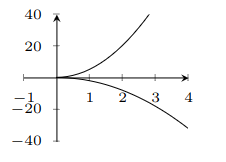
\includegraphics[width=0.35\linewidth]{plots/image.png}}

By definition, a function assigns each element of $\mathbb{X}$ to exactly one element of $\mathbb{Y}$. So this is \colorbox{yellow}{not a function}. \\

\subsection*{2. 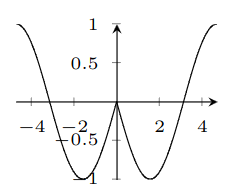
\includegraphics[width=0.35\linewidth]{plot2.png} }

This graph passes the vertical line test, so \colorbox{yellow}{it is a function}. 

\section*{Problem C}

\subsection*{$f(x) = \sqrt{2x}, g(x) = \frac{x}{x-1}$}
Write formulas for
\subsection*{1. $f + g$ and find the domain and range.}

Domains

\[
D(f) = \{ x \in \mathbb{R} \mid x \geq 0 \}
\]
\[
D(g) = \{ x \in \mathbb{R} \mid x \neq 1 \}
\]
\begin{center}
\colorbox{yellow}{$D(f+g) = \{ x \in \mathbb{R} \mid x \geq 0 \mid x \neq 1 \}$}
\end{center}

Ranges
\[
R(f) = \{ f \in \mathbb{R} \mid f \geq 0 \}
\]
\[
R(g) = \{ g \in \mathbb{R} \mid g \neq 1 \}
\]

\begin{center}
\colorbox{yellow}{Finding the range of $f + g$ is too complex.}
\end{center}
Viewing the function in Desmos, we notice a gap in the range between approximately 0.3 and 3.9. To find the exact values, we could identify the minimum from lower part and maximum from upper by taking the derivative of the sum of functions and setting it to zero. However, this leads to quartic equations, and I couldn’t fully grasp the process of obtaining the exact values. \\
I believe this complexity wasn't intended, so I won't solve it.

\subsection*{2. $f \circ g$ and find the domain and range.}

\[
(f \circ g)(x) = \sqrt{\frac{2x}{x-1}}
\]
\[
\frac{2x}{x-1} \geq 1
\]
\[
2 + \frac{2}{x-1} \geq 1
\]
The critical points are 0 and 1. The value is negative in interval $(0; 1)$, so we will exclude it

\begin{center}
\colorbox{yellow}{$D(f \circ g) = \{ x \in \mathbb{R} \mid x \leq 0 \mid x > 1 \}$}
\end{center}

The range seems all positive numbers at first, but when we look at the inner part more closely, we can proof that it can't be 2
\[
\begin{aligned}
\frac{2x}{x-1} &= 2 \\
2 + \frac{2}{x-1} &= 2 \\ 
\frac{2}{x-1} &= 0 \\
\end{aligned}
\]

Accounting the square root we get

\begin{center}
\colorbox{yellow}{$R(f \circ g) = \{ f \circ g = y \mid y \in \mathbb{R} \mid y \geq 0 \mid y \neq \sqrt{2} \}$}
\end{center}


\subsection*{3. $g \circ f$ and find the domain and range.}

\[
g(f(x)) = \frac{\sqrt{2x}}{\sqrt{2x} - 1}
\]
\[
g(f(x)) = 1 + \frac{1}{\sqrt{2x} - 1}
\]
\[
\sqrt{2x} \neq 1
\]
\[
2x \neq 1
\]
\[
x \neq 0.5
\]

\begin{center}
\colorbox{yellow}{$D(g \circ f) = \{ x \in \mathbb{R} \mid x \neq 0.5 \}$}
\end{center}

\[
\begin{aligned}
1 + \frac{1}{\sqrt{2x} - 1} \neq 1
\end{aligned}
\]

\begin{center}
\colorbox{yellow}{$R(g \circ f) = \{ f \circ g = y \mid y \in \mathbb{R} \mid y \neq 1 \}$}
\end{center}

\section*{Problem D}
$g(x) = \sqrt{\frac{1}{x-4}}$ \\
Write equations for the graphs that are obtained from the graph of g by shifting or scaling, as indicated.

\subsection*{1. Up $\frac{1}{2}$ unit, right $3$.}

To move it up we add $\frac{1}{2}$ to the result.
\[
g(x) = \sqrt{\frac{1}{x-4}} + \frac{1}{2}
\]
To move it right 3 units, we change the $x$ to be $x-3$.

\[
g(x) = \sqrt{\frac{1}{x - 3 - 4}} + \frac{1}{2}
\]

\begin{center}
\colorbox{yellow}{$g(x) = \sqrt{\frac{1}{x - 7}} + \frac{1}{2}$}
\end{center}

\subsection*{2. Compress vertically by a factor of $5$.}

To compress we multiply the result by $\frac{1}{5}$.

\begin{center}
\colorbox{yellow}{$g(x) = \sqrt{\frac{1}{x-4}} * \frac{1}{5}$}
\end{center}

\subsection*{3. Down $2$ unit, left $1$.}

To move down $2$ units, we subtract $2$ from the result.

\[
g(x) = \sqrt{\frac{1}{x-4}} - 2
\]

To move it to the left by $1$ unit, we add $1$ to $x$.

\[
g(x) = \sqrt{\frac{1}{x+1-4}} - 2
\]

\begin{center}
\colorbox{yellow}{$g(x) = \sqrt{\frac{1}{x-3}} - 2$}
\end{center}

\subsection*{4. Stretch horizontally by a factor of $3$.}

To stretch, we divide $x$ by a factor of $3$

\begin{center}
\colorbox{yellow}{$g(x) = \sqrt{\frac{1}{\frac{x}{3}-4}}$}
\end{center}

\section*{Problem E}
$f(x) = -\frac{x}{x+2}$. 
Sketch the graph of $f^{-1}$, if any. Find the domain and
range of the inverse function. \\

To find the inverse function, we can swap $x$ and $y$ around.

\[
y = -\frac{x}{x+2}
\]
\[
x = -\frac{y}{y+2}
\]
\[
\frac{y}{y+2} = -x
\]
\[
y = -x(y + 2)
\]
\[
y = -xy - 2x
\]
\[
y + xy = -2x
\]
\[
y(x + 1) = -2x
\]
\[
y = -\frac{2x}{x+1}
\]

\colorbox{yellow}{Here is the graph of the inverse function.}

\begin{center}
    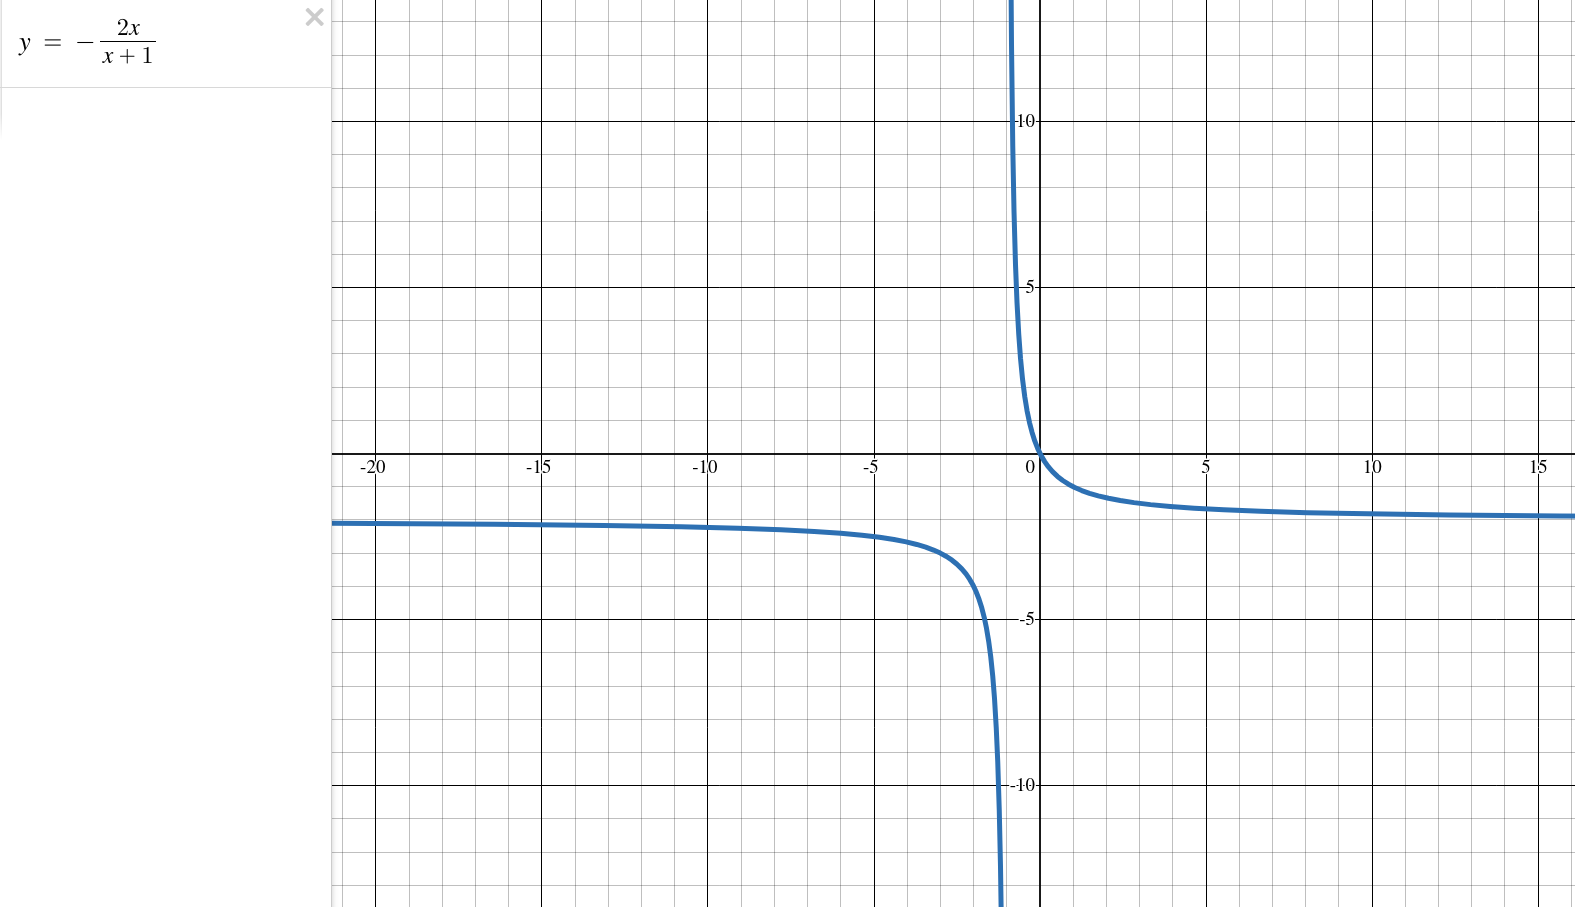
\includegraphics[width=0.8\linewidth]{graph2.png}
\end{center}

\begin{center}
\colorbox{yellow}{$D(f) = \{ x \in \mathbb{Z} \mid x \neq -1 \}$}
\end{center}

\begin{center}
\colorbox{yellow}{$R(f) = \{ f \in \mathbb{Z} \mid f \neq -2 \}$}
\end{center}

\end{document}
